\clearpage
\section{Введение}
За последние десять лет количество публикаций в сфере машинного обучения выросло примерно в 10 раз (по данным ELibrary, Arxive и ScienceOpen). Это изображено на графике (рис. \ref{intro:lit}). Данный факт говорит о росте интереса к данной области не только со стороны исследователей, но и со стороны бизнеса.
\par
\begin{figure}[h]
	\centering
	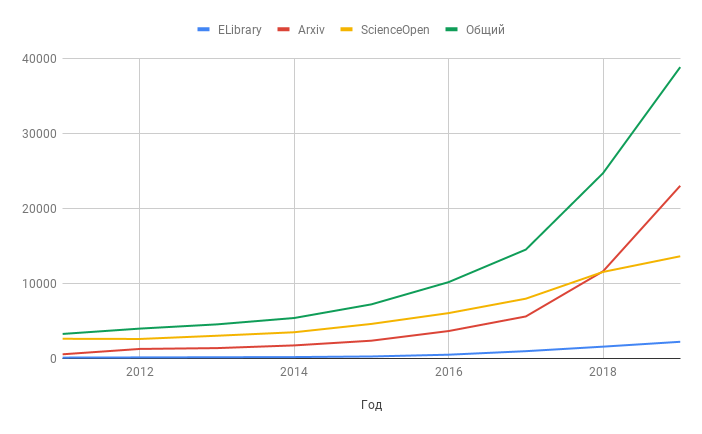
\includegraphics[width=0.9\textwidth]{ml_popularity}
	\caption{График числа публикаций с 2010 г. по 2019 г.}
	\label{intro:lit}
\end{figure}
\par
По данным отчета консалтингового агентства PricewaterhouseCoopers “Sizing the prize. What’s real value of AI and how you can capitalize it?” вклад искусственного интеллекта в мировую экономику может достигнуть 15,7 триллионов долларов США к 2030 году, что эквивалентно росту глобального ВВП на 14\%. Главными двигателями этого роста авторы называют повышение автоматизации бизнес-процессов, смешение существующей рабочей силы и новых возможностей и повышение потребительского спроса. Согласно исследованию, наибольшее влияние искусственный интеллект окажет на здравоохранение, автомобильную промышленность, финансовый сектор, логистику, сферу развлечений, розничную торговлю, энергетику и производство. Развитие новых технологий может привести к тому, что уже через 5-10 лет лидеры рынка в этой сфере окажутся в аутсайдерах, если не начнут адаптироваться к новым реальностям.
\par
Другой отчет PwC “Artificial Intelligence: Touchpoints with consumers” показывает рост интереса к искусственному интеллекту среди потребителей. Согласно их опросу, 10\% респондентов владеют устройствами с AI (роботы, умные колонки и т.д.) и ещё 32\% заявили о своем желании приобрести подобное устройство.
\par
Бурный рост интереса к искусственному интеллекту в целом и глубокому обучению в частности можно связать с увеличением доступных человечеству вычислительных ресурсов. На графике (рис. \ref{intro:perf}) видно, как росла пиковая производительность суперкомпьютеров. По оси ординат отложена производительность в TFlop/s (терафлопс, $10^12$ операций с плавающей точкой в секунду). Самый первый качественный скачок можно заметить в 2008 году. Это можно связать с появлением на рынке технологии NVidia CUDA. На графике (рис. \ref{intro:cuda}) показано, как изменялась с годами частота поискового запроса “CUDA” в поисковой системе Google. Использование графических ускорителей для вычислений позволило снизить стоимость. Кроме того, сами графические процессоры становились мощнее и дешевле. Снижение стоимости одного TFlop/s отображено на графике (рис. \ref{intro:price}). Исследовались только видеокарты NVidia. Стоимость рассчитывалась с учетом инфляции.
\begin{figure}[h]
	\centering
	\includegraphics[width=0.9\textwidth]{price}
	\caption{График снижения стоимоти 1 TFlop/s}
	\label{intro:price}
\end{figure}
\begin{figure}[h]
	\centering
	\includegraphics[width=0.9\textwidth]{perf}
	\caption{Пиковая производительность суперкомпьютеров}
	\label{intro:perf}
\end{figure}
\begin{figure}[h]
	\centering
	\includegraphics[width=0.9\textwidth]{cuda_google_trends}
	\caption{Популярность запроса CUDA в Google}
	\label{intro:cuda}
\end{figure}
